\section{Atividade 9}

\subsection{Análise do Diagrama de Nyquist}

O diagrama de Nyquist é uma ferramenta essencial para visualizar a resposta em frequência da função de transferência de malha aberta e para avaliar a estabilidade do sistema em malha fechada. A seguir, analisamos a estabilidade geral do sistema e as margens de ganho e fase, utilizando o diagrama de Nyquist para o sistema massa-mola-amortecedor com parâmetros \(M = 10\), \(C = 7\), e \(K = 5\).

\subsubsection{Diagrama de Nyquist e Estabilidade do Sistema}

\begin{figure}[H]
    \centering
    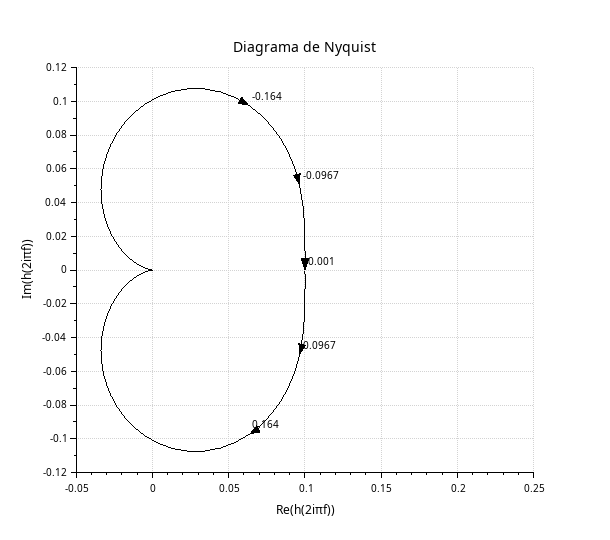
\includegraphics[width=0.8\textwidth]{atividades/9-atividade/assets/nyquist.png}
    \caption{Diagrama de Nyquist do sistema massa-mola-amortecedor.}
    \label{fig:Nyquist1}
\end{figure}

Na Figura \ref{fig:Nyquist1}, observamos que a trajetória da curva em relação ao ponto crítico \(-1 + 0j\) não circunda este ponto, indicando que o sistema é estável em malha fechada. Este comportamento sugere que o sistema não atingirá instabilidade sob condições normais de operação.

\subsubsection{Interpretação Geométrica e Estabilidade}

O diagrama mapeia a resposta complexa da função de transferência ao longo de uma gama de frequências no plano complexo. Este mapeamento é crucial para aplicar o critério de Nyquist:
\begin{itemize}
    \item A curva não encircla o ponto \(-1\), confirmando a estabilidade em malha fechada segundo o Princípio do Argumento.
    \item A proximidade da curva ao ponto crítico ajuda a determinar a margem de estabilidade antes que ganhos adicionais possam induzir instabilidade.
\end{itemize}

\subsubsection{Análise de Polos e Zeros e Margens de Ganho e Fase}

\begin{figure}[H]
    \centering
    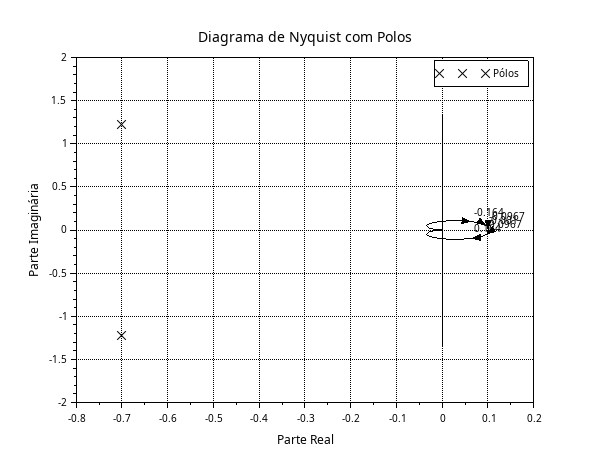
\includegraphics[width=0.8\textwidth]{atividades/9-atividade/assets/nyquist-com-polos.png}
    \caption{Diagrama de Nyquist com visualização de polos do sistema massa-mola-amortecedor.}
    \label{fig:NyquistPolos}
\end{figure}

A Figura \ref{fig:NyquistPolos} mostra a localização dos polos, marcados com 'X', no diagrama de Nyquist, oferecendo insights adicionais sobre como os polos e zeros influenciam a estabilidade e resposta do sistema:
\begin{itemize}
    \item Os polos no semiplano esquerdo confirmam a estabilidade, enquanto sua proximidade ao eixo imaginário pode indicar sensibilidade a perturbações.
    \item As margens de ganho e fase podem ser visualmente estimadas pela distância e ângulo da curva em relação ao ponto \(-1 + 0j\), sugerindo que o sistema possui uma margem de segurança robusta para tolerar variações nos parâmetros de controle.
\end{itemize}

\subsubsection{Análise Quantitativa das Margens de Ganho e Fase}
A margem de ganho é crucial para determinar quão perto o sistema está de atingir a instabilidade sob aumento de ganho. No Diagrama de Nyquist, a distância mínima do ponto \(-1 + 0j\) até a curva pode ser visualmente estimada e, em casos práticos, calculada utilizando software específico. Por exemplo, uma distância de 0.5 unidades no diagrama pode indicar que o ganho pode ser aumentado em até 50\% antes de o sistema se tornar instável.

Da mesma forma, a margem de fase é determinada calculando o ângulo que falta para que a curva passe exatamente pelo ponto \(-1 + 0j\). Um ângulo de margem de fase de 30° sugere que uma mudança de fase de até 30° ainda manteria o sistema estável. A análise detalhada dessas margens ajuda a prever e evitar cenários de instabilidade em aplicações práticas.

\subsubsection{Conclusão}
A análise combinada dos diagramas de Nyquist reforça a percepção de estabilidade do sistema, indicando amplas margens de ganho e fase. No entanto, é recomendável complementar esta análise com outras técnicas de análise de estabilidade, como diagramas de Bode ou análise de lugar das raízes, para uma avaliação mais abrangente da robustez do sistema. Essas técnicas adicionais ajudarão a confirmar as descobertas e a proporcionar uma compreensão mais completa das dinâmicas do sistema sob diferentes condições de operação.
